
\part{Số và đại số}
\chapter{CĂN BẬC HAI VÀ CĂN BẬC BA}
\section{Tính chất phép khai phương}
\subsection{Căn thức bậc hai một bình phương}
\subsubsection{Kiến thức trọng tâm}
\begin{tomtat}
Với mọi số thực $a$, ta có $\sqrt{a^2}=|a|$, cụ thể là
\begin{itemize}
\item $\sqrt{a^2}= a$ khi $a \geq 0$;
\item $\sqrt{a^2}= -a$ khi $a < 0$.
\end{itemize}
Tổng quát hơn, ta có tính chất sau đây \\
Với biểu thức $A$ bất kì, ta có $\sqrt{A^2}=| A |$, nghĩa là 
\begin{itemize}
\item $\sqrt{A^2}= A$ khi $A \geq 0$ (tức là khi $A$ nhận giá trị không âm); 
\item $\sqrt{A^2}=- A$ khi $A <0$ (tức là khi $A$ nhận giá trị âm).
\end{itemize}
\end{tomtat}

\begin{vd}%[Dự án EX-9-Đề Cương Toán 9]%[Phạm Tuấn]%[9D3N3-1]
Tính giá trị các biểu thức sau
\begin{multicols}{2}
\begin{enumerate}
\item  $\sqrt{9^2}$;
\item  $\sqrt{(-11)^2} + \sqrt{15^2}$.
\end{enumerate}
\end{multicols}
\loigiai{
\begin{enumerate}
\item  Ta có $\sqrt{9^2} = |9|=9$;
\item  Ta có $\sqrt{(-11)^2} + \sqrt{15^2} = |-11|+|15| = 11+15=26$.
\end{enumerate}
}
\end{vd}


\begin{vd}%[Dự án EX-9-Đề Cương Toán 9]%[Phạm Tuấn]%[9D3N3-1]
Rút gọn các biểu thức sau
\begin{multicols}{2}
\begin{enumerate}
\item  $\sqrt{(1-\sqrt{3})^2}+ 2\sqrt{3}+4$;
\item  $\sqrt{(2-\sqrt{5})^2}- \sqrt{5}+1$.
\end{enumerate}
\end{multicols}
\loigiai{
\begin{enumerate}
\item  Ta có $\sqrt{(1-\sqrt{3})^2}+ 2\sqrt{3}+4 = |1-\sqrt{3}|+2\sqrt{3}+4 = \sqrt{3}-1 + 2\sqrt{3}+4= 3\sqrt{3}+3$.
\item  Ta có $\sqrt{(2-\sqrt{5})^2}- \sqrt{5}+1 = |2-\sqrt{5}| - \sqrt{5}+1 = \sqrt{5}- 2 - \sqrt{5} + 1 =-1$.
\end{enumerate}
}
\end{vd}


\begin{vd}%[Dự án EX-9-Đề Cương Toán 9]%[Phạm Tuấn]%[9D3H3-1]
Rút gọn các biểu thức sau
\begin{multicols}{2}
\begin{enumerate}
\item  $\sqrt{x^4}$;
\item  $\sqrt{x^2-4x+4}$ với $x>2$.
\end{enumerate}
\end{multicols}
\loigiai{
\begin{enumerate}
\item  Vì $x^2 \geq 0$ với mọi $x$ nên  $\sqrt{x^4} = |x^2| = x^2$. 
\item  Với $x>2$,  $\sqrt{x^2-4x+4} = \sqrt{(x-2)^2} = |x-2| = x-2$.
\end{enumerate}
}
\end{vd}


\begin{vd}%[Dự án EX-9-Đề Cương Toán 9]%[Phạm Tuấn]%[9D3H3-1]
Rút gọn biểu thức $T=2\sqrt{4x^2-4x+1}+3\sqrt{x^2+2x+1}$ với $x <  -1$.
\loigiai{
Ta có 
\[
2\sqrt{4x^2-4x+1}+3\sqrt{x^2+2x+1} =2 \sqrt{(2x-1)^2}+3\sqrt{(x+1)^2} = 2|2x-1|+3|x+1|. 
\]
Với $x < -1$, $|2x-1|= 1-2x$ và $|x+1| = -(x+1)$. \\
Do đó $T= 2(1-2x)-3(x+1) = -7x-1$.
}
\end{vd}


\begin{vd}%[Dự án EX-9-Đề Cương Toán 9]%[Phạm Tuấn]%[9D3V3-1]
Tìm $x>0$ thỏa mãn $2\sqrt{x^2}+ \sqrt{x^2-6x+9} = 9$.
\loigiai{
Ta có 
\begin{eqnarray*}
&& 2\sqrt{x^2}+ \sqrt{x^2-6x+9} = 9 \\
&& 2|x|+|x-3|=9.
\end{eqnarray*}
Ta xét hai trường hợp
\begin{itemize}
\item $0<x<3$, khi đó 
\begin{eqnarray*}
&& 2|x|+|x-3|=9 \\
&& 2x+3-x =9 \\
&& x=6 ~ (\text{loại}).
\end{eqnarray*}
\item $x \geq  3$, khi đó 
\begin{eqnarray*}
&& 2|x|+|x-3|=9 \\
&& 2x+x-3 =9 \\
&& x=4.
\end{eqnarray*}
\end{itemize}
Vậy $x=4$.
}
\end{vd}

\subsubsection{Bài tập}

\begin{bt}%[Dự án EX-9-Đề Cương Toán 9]%[Phạm Tuấn]%[9D3N3-1]
Tính giá trị biểu thức
\begin{multicols}{2}
\begin{enumerate}
\item  $A=\sqrt{81}+\sqrt{(-6)^2}$;
\item  $B =-\sqrt{\left(-\frac{4}{11}\right)^2}+\left(-\sqrt{\frac{15}{11}}\right)^2$.
\end{enumerate}
\end{multicols}
\loigiai{
\begin{enumerate}
\item  Ta có $A=\sqrt{81}+\sqrt{(-6)^2} = \sqrt{8^2}+\sqrt{(-6)^2} = |8|+ |-6| = 14$.
\item  Ta có $B =-\sqrt{\left(-\frac{4}{11}\right)^2}+\left(-\sqrt{\dfrac{15}{11}}\right)^2 = - \left |-\dfrac{4}{11} \right | + \dfrac{15}{11} =-\dfrac{4}{11}+ \dfrac{15}{11} = 1$.
\end{enumerate}
}
\end{bt}


\begin{bt}%[Dự án EX-9-Đề Cương Toán 9]%[Phạm Tuấn]%[9D3H3-1]
Tính giá trị biểu thức
\begin{enumerate}
\item  $A= \sqrt{(4-\sqrt{11})^2}+\sqrt{(3-\sqrt{11})^2}$; 
\item  $B =2\sqrt{(\sqrt{3}-6)^2}+ \sqrt{(1-\sqrt{3})^2} - 2 \sqrt{(4-\sqrt{3})^2}$.
\end{enumerate}
\loigiai{
\begin{enumerate}
\item  $A= \sqrt{(4-\sqrt{11})^2}+\sqrt{(3-\sqrt{11})^2} = |4-\sqrt{11}|+|3-\sqrt{11}| = 4-\sqrt{11}+\sqrt{11}-3 =1$.
\item  Ta có
\begin{eqnarray*}
B &&=2\sqrt{(\sqrt{3}-6)^2}+ \sqrt{(1-\sqrt{3})^2} - 2 \sqrt{(4-\sqrt{3})^2}\\
&&= 2|\sqrt{3}-6|+ |1-\sqrt{3}|-2|4-\sqrt{3}| \\
&&=2(6-\sqrt{3})+ \sqrt{3}-1 -2 (4-\sqrt{3}) \\
&&=3+\sqrt{3}.
\end{eqnarray*}
\end{enumerate}
}
\end{bt}


\begin{bt}%[Dự án EX-9-Đề Cương Toán 9]%[Phạm Tuấn]%[9D3H3-1]
Rút gọn các biểu thức sau
\begin{multicols}{2}
\begin{enumerate}
\item  $\sqrt{x^8}$;
\item  $\sqrt{25x^2-10x+1}$ với $x < \dfrac{1}{5}$.
\end{enumerate}
\end{multicols}
\loigiai{
\begin{enumerate}
\item  Vì $x^4 \geq 0$ với mọi $x$ nên  $\sqrt{x^8} =\sqrt{(x^4)^2}  = |x^4| = x^4$. 
\item  Với $x< \dfrac{1}{5}$, $5x-1 <0$. \\
 Do đó   $\sqrt{25x^2-10x+1} = \sqrt{(5x-1)^2} = |5x-1| = 1-5x$.
\end{enumerate}
}
\end{bt}

\begin{bt}%[Dự án EX-9-Đề Cương Toán 9]%[Phạm Tuấn]%[9D3H3-1]
Rút gọn các biểu thức sau
\begin{multicols}{2}
\begin{enumerate}
\item  $4\sqrt{a^2}-2a$ với $a <0$;
\item  $2a+3 - \sqrt{a^2-4a+2}$ với $a \geq  2$.
\end{enumerate}
\end{multicols}
\loigiai{
\begin{enumerate}
\item Với $a<0$, ta có $4\sqrt{a^2}-2a = 4|a|-2a =-4a-2a = -6a$.
\item Với $a \geq 2$, ta có 
\[
2a+3 - \sqrt{a^2-4a+2} = 2a+3 -\sqrt{(a-2)^2} = 2a+3 - |a-2|=2a+3 - (a-2) = a+5.
\]
\end{enumerate}
}
\end{bt}

\begin{bt}%[Dự án EX-9-Đề Cương Toán 9]%[Phạm Tuấn]%[9D3V3-1]
Rút gọn biểu thức $T= \sqrt{4a^2-4a+1}+\sqrt{a^2+6a+9}$ với $-3<a<\dfrac{1}{3}$.
\loigiai{
Ta có 
\begin{eqnarray*}
T&&= \sqrt{9a^2-6a+1}+\sqrt{a^2+6a+9} \\
&&= \sqrt{(3a-1)^2} + \sqrt{(a+3)^2} \\
&& = |3a-1|+ |a+3|.
\end{eqnarray*}
Khi $-3<a<\dfrac{1}{3}$, ta có $|3a-1| = 1-3a$, $|a+3| = a+3$. \\
Do đó $T= 1-3a+a+3 = -2a+4$.
}
\end{bt}

\begin{bt}%[Dự án EX-9-Đề Cương Toán 9]%[Phạm Tuấn]%[9D3V3-1]
Tìm $x<0$ thỏa mãn $\sqrt{x^2+4x+4}- 2\sqrt{x^2} = -1$.
\loigiai{
Ta có 
\begin{eqnarray*}
&& \sqrt{x^2+4x+4}- 2\sqrt{x^2} = -1\\
&& \sqrt{(x+2)^2}- 2\sqrt{x^2} = -1\\
&& |x+2|-2|x|=-1.
\end{eqnarray*}
Ta xét hai trường hợp
\begin{itemize}
\item $-2<x<0$, khi đó 
\begin{eqnarray*}
&& |x+2|-2|x|=-1\\
&& x+2+2x =-1 \\
&& x=-1 ~ (\text{thỏa mãn}).
\end{eqnarray*}
\item $x \leq -2$, khi đó 
\begin{eqnarray*}
&& |x+2|-2|x|=-1 \\
&& -x-2+2x =-1 \\
&& x=1 ~ (\text{loại}).
\end{eqnarray*}
\end{itemize}
Vậy $x=-1$.
}
\end{bt}



\subsection{Căn thức bậc hai một tích}
\subsubsection{Kiến thức trọng tâm}
\begin{tomtat}
\begin{itemize}
\item Với hai số thực $a$ và $b$ không âm, ta có $\sqrt{ a \cdot b }=\sqrt{ a } \cdot \sqrt{ b }$. 
\item Tổng quát hơn, ta có tính chất sau đây\\
Với hai biểu thức $A$ và $B$ nhận giá trị không âm, ta có $\sqrt{A \cdot B}=\sqrt{A} \cdot \sqrt{B}$.
\item Đưa thừa số ra ngoài dấu căn. \\
Với số thực $a$ bất kì và $b$ không âm, ta có $\sqrt{a ^2b}=|a|\sqrt{b}$.
\item Đưa thừa số vào trong dấu căn. \\
Nếu $a\geq 0$ thì $a \sqrt{b}=\sqrt{a^2 b}$;  nếu $a<0$ thì $a \sqrt{b}=-\sqrt{a^2b}$.
\end{itemize}
\begin{luuy}
Với các biểu thức $A$, $B$ và $C$ nhận giá trị không âm, ta có $\sqrt{A \cdot B \cdot C}=\sqrt{A} \cdot \sqrt{B} \cdot \sqrt{C}$.
\end{luuy}
\end{tomtat}


\begin{vd}%[Dự án EX-9-Đề Cương Toán 9]%[Phạm Tuấn]%[9D3N3-2]
Tính giá trị các biểu thức 
\begin{multicols}{2}
\begin{enumerate}
\item  $\sqrt{25 \cdot 11^2}$;
\item  $\sqrt{20 \cdot 120}$.
\end{enumerate}
\end{multicols}
\loigiai{
\begin{enumerate}
\item  Ta có $\sqrt{25 \cdot 11^2} = \sqrt{25} \cdot \sqrt{11^2} = 5 \cdot 11 =55$.
\item  Ta có $\sqrt{30 \cdot 120} = \sqrt{3 \cdot 12 \cdot 10 \cdot 10} = \sqrt{36 \cdot 100} = \sqrt{36} \cdot \sqrt{100} = 6 \cdot 10 =36$.
\end{enumerate}
}
\end{vd}

\begin{vd}%[Dự án EX-9-Đề Cương Toán 9]%[Phạm Tuấn]%[9D3H3-2]
Tính giá trị các biểu thức 
\begin{multicols}{2}
\begin{enumerate}
\item  $2\sqrt{20}+ \sqrt{45}$;
\item  $3\sqrt{12}+ 2\sqrt{27}- \sqrt{75}$.
\end{enumerate}
\end{multicols}
\loigiai{
\begin{enumerate}
\item  Ta có $2\sqrt{20}+ \sqrt{45} = 2\sqrt{2^2 \cdot 5} + \sqrt{3^2 \cdot 5} = 4 \sqrt{5} + 3\sqrt{5} = 7\sqrt{5}$;
\item  Ta có $3\sqrt{12}+ 2\sqrt{27}- \sqrt{75} = 3\sqrt{2^2 \cdot 3} + 2\sqrt{3^2 \cdot 3} - \sqrt{5^2 \cdot 3} = 6\sqrt{3}+6\sqrt{3}-5\sqrt{3}=-5\sqrt{3}$.
\end{enumerate}
}
\end{vd}

\begin{vd}%[Dự án EX-9-Đề Cương Toán 9]%[Phạm Tuấn]%[9D3H3-2]
Đưa các thừa số vào bên trong dấu căn
\begin{multicols}{2}
\begin{enumerate}
\item  $5\sqrt{8}$;
\item  $-3\sqrt{10}$;
\item  $x\sqrt{8y}$ với $x \geq 0$;
\item  $2x \sqrt{3y^2}$ với $x<0$.
\end{enumerate}
\end{multicols}
\loigiai{
\begin{enumerate}
\item $5\sqrt{8} = \sqrt{5^2 \cdot 8} = \sqrt{200}$.
\item $-3\sqrt{10} = - \sqrt{3^2 \cdot 10} = - \sqrt{90}$.
\item Với $x \geq 0$, $x\sqrt{8y} = \sqrt{8x^2y}$.
\item Với $x<0$, $2x \sqrt{3y^2} = - \sqrt{(2x)^2 \cdot 3y^2} = - \sqrt{12x^2y^2}$.
\end{enumerate}
}
\end{vd}


\begin{vd}%[Dự án EX-9-Đề Cương Toán 9]%[Phạm Tuấn]%[9D3H3-2]
Rút gọn biểu thức 
\begin{multicols}{2}
\begin{enumerate}
\item   $\sqrt{7 x } \cdot \sqrt{28 x }$ với $x \geq 0$;
\item   $\sqrt{6 x^2} \cdot \sqrt{8x} \cdot \sqrt{3 y^2}$ với $x>0$ và $y<0$.
\end{enumerate}
\end{multicols}
\loigiai{
\begin{enumerate}
\item  Ta có $\sqrt{7 x } \cdot \sqrt{28 x} = \sqrt{196 x^2} =\sqrt{(14x)^2}= |14x| =14x$.
\item  Ta có $\sqrt{6 x^2} \cdot \sqrt{8x} \cdot \sqrt{3x y^2} = \sqrt{6 x^2 \cdot 8x \cdot 3x y^2} = \sqrt{\left (12x^2y\right )^2} = |12x^2y| = -12x^2y$.
\end{enumerate}
}
\end{vd}

\begin{vd}%[Dự án EX-9-Đề Cương Toán 9]%[Phạm Tuấn]%[9D3H3-2]
Một hình chữ nhật có chiều dài là $\sqrt{\dfrac{a}{3}}$ mét và chiều rộng là $\sqrt{\dfrac{a}{12}}$ mét $(a>0)$. Tính diện tích của hình chữ nhật theo $a$.
\loigiai{
Diện tích của hình chữ nhật là 
\[
S= \sqrt{\dfrac{a}{3}} \cdot  \sqrt{\dfrac{a}{12}} = \sqrt{\dfrac{a}{3} \cdot \dfrac{a}{12}} = \sqrt{\left (\dfrac{a}{6}\right )^2} =  \dfrac{a}{6} ~ (\text{m}^2).
\]
}
\end{vd}

\begin{vd}%[Dự án EX-9-Đề Cương Toán 9]%[Phạm Tuấn]%[9D3V3-2]
Cho tam giác $ABC$ đều có đường cao $AH$. Biết $AH=6\sqrt{6}$ cm, tính diện tích tam giác $ABC$.
\loigiai{
\immini{
Đặt $AB =2x$ (cm).  \\
Trong tam giác đều đường cao cũng là đường trung tuyến nên 
$$BH= \dfrac{1}{2} BC = \dfrac{1}{2} AB =x.$$
Áp dụng định lý Pythagore $AB^2 = AH^2 + BH^2$.
}
{
\begin{tikzpicture}[scale=1,>=stealth, font=\footnotesize, line join=round, line cap=round]
\path
(0,0) coordinate (A)
(-120:3) coordinate (B)
(-60:3) coordinate (C)
($(B)!0.5!(C)$) coordinate (H)
;
\draw (A)--(B)--(C)--(A)--(H)   ;
\foreach \x/\g in {A/90,B/-140,C/-40,H/-90}
\fill[black] (\x) circle(1.1pt) + (\g:4mm) node {$\x$};
\end{tikzpicture}
}
Suy ra 
\begin{eqnarray*}
&&  4x^2=x^2+ (6\sqrt{6})^2 \\
&&  3x^2 =  216 \\
&& x^2 = 72 \\
&& x= 6\sqrt{2}. 
\end{eqnarray*}
Diện tích tam giác $ABC$ là 
\[
S= \dfrac{1}{2} AH \cdot BC = \dfrac{1}{2} \cdot 6\sqrt{6} \cdot  12 \sqrt{2} =   72\sqrt{3} ~(\text{cm}^2).
\]
}
\end{vd}


\begin{vd}%[Dự án EX-9-Đề Cương Toán 9]%[Phạm Tuấn]%[9D3V3-2]
Rút gọn các biểu thức 
\begin{multicols}{2}
\begin{enumerate}
\item  $\sqrt{19-8\sqrt{3}} + \sqrt{4-2\sqrt{3}}$;  
\item  $2\sqrt{11-6\sqrt{2}} + \sqrt{9-4\sqrt{2}}$.
\end{enumerate}
\end{multicols}
\loigiai{
\begin{enumerate}
\item  Ta có
\begin{eqnarray*}
\sqrt{19-8\sqrt{3}} + \sqrt{4-2\sqrt{3}} &&= \sqrt{4^2-2 \cdot 4 \cdot \sqrt{3}+ (\sqrt{3})^2}  + \sqrt{1^2-2 \cdot 1 \cdot \sqrt{3}+ (\sqrt{3})^2}\\
&& = \sqrt{(4-\sqrt{3})^2} + \sqrt{(1-\sqrt{3})^2}  \\
&&= |4-\sqrt{3}|+|1-\sqrt{3}| \\
&& = 4-\sqrt{3} + \sqrt{3} -1 \\
&&=3.
\end{eqnarray*}
\item  Ta có
\begin{eqnarray*}
2\sqrt{11-6\sqrt{2}} + \sqrt{9-4\sqrt{2}} &&= 2\sqrt{3^2-2 \cdot 3 \cdot \sqrt{2}+ (\sqrt{2})^2}  + \sqrt{1^2-2 \cdot 1 \cdot 2\sqrt{2}+ (2\sqrt{2})^2}\\
&& = 2\sqrt{(3-\sqrt{2})^2} + \sqrt{(1-\sqrt{2})^2}  \\
&&= 2|3-\sqrt{2}|+|1-\sqrt{2}| \\
&& = 2(3-\sqrt{2}) + \sqrt{2} -1 \\
&&=5-\sqrt{2}.
\end{eqnarray*}
\end{enumerate}
}
\end{vd}





\begin{vd}%[Dự án EX-9-Đề Cương Toán 9]%[Phạm Tuấn]%[9D3V3-2]
Cho $x$, $y$ là hai số thực không âm. Chứng minh rằng $x+ y \geq 2\sqrt{xy}$.
\loigiai{
Ta có 
$$x+y-2\sqrt{xy} = (\sqrt{x})^2 - 2\sqrt{x} \cdot \sqrt{y} + (\sqrt{y})^2 = (\sqrt{x}-\sqrt{y})^2 \geq 0$$
với mọi $x$, $y$ là hai số thực không âm. \\
Suy ra $x+ y \geq 2\sqrt{xy}$.
}
\end{vd}
\subsubsection{Bài tập}


\begin{bt}%[Dự án EX-9-Đề Cương Toán 9]%[Phạm Tuấn]%[9D3H3-2]
Tính giá trị các biểu thức 
\begin{multicols}{2}
\begin{enumerate}
\item  $\sqrt{10} \cdot \sqrt{40}$;
\item  $\sqrt{4} \cdot \sqrt{5} \cdot \sqrt{80}$;
\item  $(8 \sqrt{6}) \cdot(-2 \sqrt{24})$;
\item  $\sqrt{\left(-\frac{7}{5}\right)^2} \cdot \sqrt{0{,}25}$;
\item  $\sqrt{\dfrac{16}{121} \cdot 125}$;
\item  $\sqrt{15 \cdot  45 \cdot 27}$.
\end{enumerate}
\end{multicols}
\loigiai{
\begin{enumerate}
\item  $\sqrt{10} \cdot \sqrt{40}=\sqrt{10\cdot40}=\sqrt{400}=\sqrt{20^2}=20$.
\item  $\sqrt{4} \cdot \sqrt{5} \cdot \sqrt{80}=\sqrt{2^2} \cdot \sqrt{5} \cdot \sqrt{4^2\cdot5}=2 \cdot \sqrt{5} \cdot \sqrt{4^2}\cdot\sqrt{5}=2 \cdot (\sqrt{5})^2 \cdot 4=40$.
\item  $(8 \sqrt{6}) \cdot(-2 \sqrt{24}) =(8 \sqrt{6}) \cdot(-4 \sqrt{6}) = -32 \cdot 6 = -198$.
\item  Ta có $\sqrt{\dfrac{16}{121} \cdot 25} = \sqrt{\left (\dfrac{4}{11}\right )^2 \cdot 5^2} = \dfrac{4}{11} \cdot 5 = \dfrac{20}{11}$.
\item  Ta có $\sqrt{15 \cdot  45 \cdot 27} = \sqrt{15^2 \cdot 9^2} = \sqrt{15^2} \cdot \sqrt{9^2} =15 \cdot 9 = 135$.
\item  $\sqrt{\left(-\dfrac{7}{5}\right)^2} \cdot \sqrt{0{,}25}=\sqrt{\left(\dfrac{7}{5}\right)^2} \cdot \sqrt{0{,}5^2}=\dfrac{7}{5}\cdot0{,}5=\dfrac{7}{5}\cdot\dfrac{5}{10}=\dfrac{7}{10}$.
\end{enumerate}
}
\end{bt}


\begin{bt}%[Dự án EX-9-Đề Cương Toán 9]%[Phạm Tuấn]%[9D3H3-2]
Tính giá trị các biểu thức 
\begin{multicols}{2}
\begin{enumerate}
\item  $\sqrt{600} \cdot \sqrt{11^2-5^2}$; 
\item  $\sqrt{\sqrt{7}+3} \cdot \sqrt{3-\sqrt{7}}$.
\end{enumerate}
\end{multicols}
\loigiai{
\begin{enumerate}
\item  Ta có $\sqrt{600} \cdot \sqrt{11^2-5^2} = \sqrt{600(11+5)(11-5)} = \sqrt{6^2 \cdot 4^2 \cdot 10^2}= 6 \cdot 4 \cdot 10 = 240$.
\item  Ta có $\sqrt{\sqrt{7}+3} \cdot \sqrt{3-\sqrt{7}}= \sqrt{(\sqrt{7}+3)(3-\sqrt{7})} = \sqrt{3^2-7} =\sqrt{2}$.
\end{enumerate}
}
\end{bt}


\begin{bt}%[Dự án EX-9-Đề Cương Toán 9]%[Phạm Tuấn]%[9D3H3-2]
Rút gọn biểu thức 
\begin{multicols}{2}
\begin{enumerate}
\item  $\sqrt{20}-\sqrt{45}+\sqrt{5}$; 
\item  $\sqrt{32}-\sqrt{200}+\sqrt{50}$; 
\item  $(\sqrt{6}-\sqrt{5})^2+\sqrt{120}$;
\item  $2(\sqrt{3}-\sqrt{2})^2+\sqrt{96}$.
\end{enumerate}
\end{multicols}
\loigiai{
\begin{enumerate}
\item  $\sqrt{20}-\sqrt{45}+\sqrt{5} =2\sqrt{5}-3\sqrt{5}+\sqrt{5} = 0$.
\item  $\sqrt{32}-\sqrt{200}+\sqrt{50} = 4\sqrt{2}-10\sqrt{2}+5\sqrt{2} = -\sqrt{2}$.
\item  $(\sqrt{6}-\sqrt{5})^2+\sqrt{120} = 6-2\sqrt{30}+5 - 2\sqrt{30} = 11$.
\item  $2(\sqrt{3}-\sqrt{2})^2+\sqrt{96} = 2(3-2\sqrt{6}+2) + \sqrt{96} = 10- \sqrt{96}+\sqrt{96}=10$.
\end{enumerate}
}
\end{bt}

\begin{bt}%[Dự án EX-9-Đề Cương Toán 9]%[Phạm Tuấn]%[9D3V3-2]
Rút gọn các biểu thức 
\begin{multicols}{2}
\begin{enumerate}
\item  $\sqrt{27-10\sqrt{2}}+\sqrt{2}$;
\item  $\sqrt{9-4\sqrt{5}}-\sqrt{5}$;
\item  $\sqrt{4+2\sqrt{3}} + \sqrt{12-6\sqrt{3}}$;
\item  $\sqrt{8-2\sqrt{7}} - \sqrt{11+4\sqrt{7}}$.
\end{enumerate}
\end{multicols}
\loigiai{
\begin{enumerate}
\item $\sqrt{27-10\sqrt{2}} = \sqrt{5^2-2 \cdot 5 \cdot \sqrt{2} +(\sqrt{2})^2} = \sqrt{(5-\sqrt{2})^2} = |5-\sqrt{2}|= 5-\sqrt{2}$. \\
Suy ra $\sqrt{27-10\sqrt{2}}+\sqrt{2} = 5$.
\item $\sqrt{9-4\sqrt{5}}= \sqrt{2^2-2 \cdot 2 \cdot \sqrt{5} +(\sqrt{5})^2} = \sqrt{(2-\sqrt{5})^2} = |2-\sqrt{5}|=\sqrt{5} -2$. \\
Suy ra $\sqrt{9-4\sqrt{5}}-\sqrt{5} = -2$.
\item  Ta có
\begin{eqnarray*}
\sqrt{4+2\sqrt{3}} + \sqrt{12-6\sqrt{3}} &&= \sqrt{1^2+2 \cdot 1 \cdot \sqrt{3}+ (\sqrt{3})^2}  + \sqrt{3^2-2 \cdot 3 \cdot \sqrt{3}+ (\sqrt{3})^2}\\
&& = \sqrt{(1+\sqrt{3})^2} + \sqrt{(3-\sqrt{3})^2}  \\
&&= |1+\sqrt{3}|+|3-\sqrt{3}| \\
&& = 1+\sqrt{3} + 3- \sqrt{3} \\
&&=4.
\end{eqnarray*}
\item  Ta có
\begin{eqnarray*}
\sqrt{8-2\sqrt{7}} - \sqrt{11+4\sqrt{7}}&&= \sqrt{1^2-2 \cdot 1 \cdot \sqrt{7}+ (\sqrt{7})^2}  - \sqrt{2^2+2 \cdot 2\cdot \sqrt{7}+ (\sqrt{7})^2}\\
&& = \sqrt{(1-\sqrt{7})^2} - \sqrt{(2+\sqrt{7})^2}  \\
&&= |1-\sqrt{7}|-|2+\sqrt{7}| \\
&& = \sqrt{7}-1-2-\sqrt{7} \\
&&=-3.
\end{eqnarray*}
\end{enumerate}
}
\end{bt}

\begin{bt}%[Dự án EX-9-Đề Cương Toán 9]%[Phạm Tuấn]%[9D3H3-2]
Rút gọn các biểu thức 
\begin{multicols}{2}
\begin{enumerate}
\item  $\sqrt{8x^3} \cdot  \sqrt{18 x}$ với $x>0$;
\item  $\sqrt{\frac{7 z}{3}} \cdot \sqrt{\frac{3}{28 z}}$ với $z>0$;
\item  $\sqrt{5 a} \cdot \sqrt{15 b} \cdot \sqrt{27 a b}$ $(a \geq 0, b \geq 0)$;
\item  $\sqrt{81x^4(2-y)^2}$ với $y \geq 2$.
\end{enumerate}
\end{multicols}
\loigiai{
\begin{enumerate}
\item  $\sqrt{8x^3} \cdot  \sqrt{18x} = \sqrt{8 \cdot 18 \cdot x^4} =\sqrt{(12x^2)^2} = 12x^2$.
\item  $\sqrt{\frac{7 z}{3}} \cdot \sqrt{\frac{3}{28 z}} = \sqrt{\frac{7 z}{3} \cdot \frac{3}{28 z}} = \sqrt{\dfrac{1}{4}}= \dfrac{1}{2}$.
\item  $\sqrt{5a} \cdot \sqrt{15b} \cdot \sqrt{27ab} = \sqrt{5^2 \cdot 9^2 \cdot (ab)^2} = 5 \cdot 9 \cdot ab = 45ab$.
\item  $\sqrt{81x^4(2-y)^2}= \sqrt{81} \cdot \sqrt{x^4} \cdot \sqrt{(2-y)^2} = 9x^2|2-y|=9x^2(y-2)$.
\end{enumerate}
}
\end{bt}

\begin{bt}%[Dự án EX-9-Đề Cương Toán 9]%[Phạm Tuấn]%[9D3H3-4]
Một hình chữ nhật có chiều dài và chiều rộng lần lượt là $\sqrt{32}$ m và $\sqrt{72}$ m. Tính diện tích của hình chữ nhật.
\loigiai{
Diện tích của hình chữ nhật là $S= \sqrt{32} \cdot \sqrt{72} =4\sqrt{2} \cdot 6\sqrt{2} = 48$ (m$^2$).
}
\end{bt}


\begin{bt}%[Dự án EX-9-Đề Cương Toán 9]%[Phạm Tuấn]%[9D3H3-2]
Một hình chữ nhật có chiều rộng và độ dài đường chéo lần lượt là $\sqrt{18}$ cm và $12$ cm . Tính diện tích của hình chữ nhật.
\loigiai{
Gọi chiều dài của hình chữ nhật là $x$ cm ($x >0$). \\
Áp dụng định lí Pythagore,  ta nhận được $x^2 = 12^2 - (\sqrt{18})^2 = 126$. Suy ra $x= \sqrt{126}$. \\
Diện tích của hình chữ nhật là
\[
S= \sqrt{18} \cdot \sqrt{126} =  \sqrt{18} \cdot \sqrt{18} \cdot \sqrt{7} = 18\sqrt{7} ~(\text{cm}^2).
\]
}
\end{bt}

\begin{bt}%[Dự án EX-9-Đề Cương Toán 9]%[Phạm Tuấn]%[9D3V3-2]
\immini{
Cho hai hình vuông $ABCD$ và $BEFG$ (hình vẽ) có $AB=8$ cm, $BE=4$ cm. Tính diện tích tam giác $BDF$.
}
{
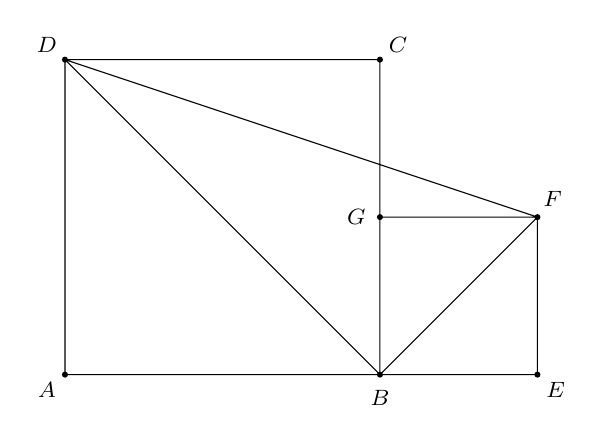
\begin{tikzpicture}[scale=1,>=stealth, font=\footnotesize, line join=round, line cap=round]
\path
(0,0) coordinate (A)
(4,0) coordinate (B)
(4,4) coordinate (C)
(0,4) coordinate (D)
(6,0) coordinate (E)
(6,2) coordinate (F)
(4,2) coordinate (G)
;
\draw (A)--(B)--(C)--(D)--(A) (B)--(E)--(F)--(G)  (D)--(B)--(F)--(D) ;
\foreach \x/\g in {A/-140,B/-90,C/40,D/140,E/-40,F/50,G/-180}
\fill[black] (\x) circle(1.1pt) + (\g:3mm) node {$\x$};
\end{tikzpicture}
}
\loigiai{
Áp dụng định lí Pythagore ta có $BD= \sqrt{8^2+8^2}= 8\sqrt{2}$ cm; $BF= \sqrt{4^2+4^2}= 4\sqrt{2}$ cm. \\
Ta lại có $\widehat{DBF} = 45^\circ+ 45^\circ =90^\circ$ nên tam giác $BDF$ vuông tại $B$. \\
Diện tích tam giác $BDF$ là $\dfrac{1}{2} BD \cdot BF = \dfrac{1}{2} \cdot 8 \sqrt{2} \cdot 4 \sqrt{2} = 64$ cm$^2$.
}
\end{bt}

\begin{bt}%[Dự án EX-9-Đề Cương Toán 9]%[Phạm Tuấn]%[9D3V3-2]
\immini{
Cho hình vẽ bên. Biết $ABCD$ là hình vuông có diện tích bằng $12$, $CMNF$ là hình vuông có diện tích bằng $27$. Tính diện tích hình chữ nhật $CDEF$.
}
{
\begin{tikzpicture}[scale=1,>=stealth, font=\footnotesize, line join=round, line cap=round]
\path
(0,4) coordinate (A)
(1.5,4) coordinate (B)
(1.5,2.5) coordinate (C)
(0,2.5) coordinate (D)
(0,0) coordinate (E)
(1.5,0) coordinate (F)
(4,2.5) coordinate (M)
(4,0) coordinate (N)
;
\draw (F)--(E)--(A)--(B)--(F)--(N)--(M)--(D) ;
\foreach \x/\g in {A/140,B/40,C/40,D/180,E/-140,F/-90,M/40,N/-40}
\fill[black] (\x) circle(1.1pt) + (\g:3mm) node {$\x$};
\end{tikzpicture}
}
\loigiai{
Diện tích hình vuông $ABCD$ bằng $12$ nên $CD^2=12$ hay $CD=\sqrt{12}=2\sqrt{3}$. \\
Diện tích hình vuông $CMNF$ bằng $27$ nên $CF^2=27$ hay $CF=\sqrt{27}=3\sqrt{3}$. \\
Diện tích hình chữ nhật $CDEF$  là $2\sqrt{3} \cdot 3\sqrt{3} = 18$.
}
\end{bt}


\begin{bt}%[Dự án EX-9-Đề Cương Toán 9]%[Phạm Tuấn]%[9D3V3-2]
.\begin{enumerate}
\item Cho $x$, $y$ là hai số thực không âm. Chứng minh rằng $4x+ 9y \geq 12\sqrt{xy}$.
\item Cho $a$, $b$, $c$ là các số thực không âm. Chứng minh rằng $a+b+c \geq \sqrt{ab} + \sqrt{bc}+\sqrt{ca}$. 
\end{enumerate}
\loigiai{
\begin{enumerate}
\item 
Ta có 
$$4x+9y-12\sqrt{xy} = (2\sqrt{x})^2 - 2 \cdot 2\sqrt{x} \cdot 3\sqrt{y} + (3\sqrt{y})^2 = (2\sqrt{x}-3\sqrt{y})^2 \geq 0$$
với mọi $x$, $y$ là hai số thực không âm. \\
Suy ra $4x+ 9y \geq 12\sqrt{xy}$.
\item Ta có 
\[
2(a+b+c) -  2\sqrt{ab} - 2\sqrt{bc}- 2\sqrt{ca}  = (\sqrt{a}- \sqrt{b})^2  + (\sqrt{b}- \sqrt{c})^2 + (\sqrt{c}- \sqrt{a})^2 \geq 0
\]
với mọi $a$, $b$, $c$ là các số thực không âm. \\
Suy ra $a+b+c \geq \sqrt{ab} + \sqrt{bc}+\sqrt{ca}$.
\end{enumerate}
}
\end{bt}
